\documentclass{standalone}
\usepackage{tikz,amsmath,graphicx}
\usepackage[update,verbose=false]{epstopdf}
\usepackage[version=3]{mhchem}
\graphicspath{{./figs/}}
\newlength{\tikzunit}
\newcommand{\scale}{.7}
\usetikzlibrary{
    arrows,
    decorations.pathmorphing,
    backgrounds,
    positioning,
    fit,
    petri
}

\begin{document}
\setlength{\tikzunit}{\textwidth/20}
\begin{tikzpicture}
    [scale=1,
     structure/.style={rectangle,draw=white,fill=white,
               outer xsep=.2cm,outer ysep=.2cm,minimum size=4mm,node distance=2cm},
     arrow/.style={->,>=stealth',semithick},
     reagent/.style={text width=2cm,font=\footnotesize,align=center,midway},
     label/.style={rectangle,fill=white,font=\bfseries,
               outer ysep=.2cm,minimum size=4mm,},
     designbox/.style={rectangle,draw=black,thick,fill=red,
               inner sep=0pt,minimum width=15mm, minimum height=2.5mm, node distance=0mm}]
    %
    \node (0) {};
    \node[structure] (init) [above=of 0, anchor=south,xshift=.7cm]
        {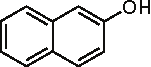
\includegraphics[scale=.9]{scheme1.pdf}};
    %
    \node[structure] (1) [base right=of init]
        {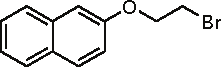
\includegraphics[scale=.9]{scheme3.pdf}};
    %
    \node[structure] (2) [base right=of 1]
        {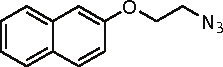
\includegraphics[scale=.9]{scheme4.pdf}};
    %
    \node[structure] (3) [right=of 0]
        {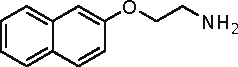
\includegraphics[scale=.9]{scheme5.pdf}};
    %
    \node[structure] (4) [right=of 3]
        {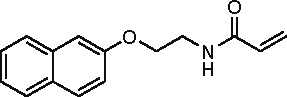
\includegraphics[scale=.9]{scheme7.pdf}};
    %
    \draw [arrow] (init) -- (1) 
        node [above,reagent]
            {
\includegraphics[scale=\scale]{scheme2.pdf} \ce{K2CO3}}
        node [below,reagent]{Acetone refulx, $24\,\mathrm{h}$};
    \draw [arrow] (1)    -- (2)
        node [above,reagent]{\ce{NaN3}}
        node [below,reagent]{DMF, $50\,\mathrm{^\circ C}, 24\,\mathrm{h}$};
    \draw [arrow] (0)    -- (3)
        node [above,reagent]{\ce{NaBH4} \ce{HTMPB} (cat.)}
        node [below,reagent]{
            \ce{H2O}/Toluene $70\,\mathrm{^\circ C}, 16\,\mathrm{h}$};
    \draw [arrow] (3)    -- (4)
        node [above,reagent]
            {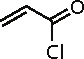
\includegraphics[scale=\scale]{scheme6.pdf}\\ \ce{TEA}}
        node [below,reagent]{\ce{CHCl3}\\ $0\,\mathrm{^\circ C}$ to rt, $4\,\mathrm{h}$};
    %
    \node[designbox] (initbox) [below=of init.south,anchor=center] {};
    \node[designbox] (4box) [below=of 4.south,anchor=center] {};
    \draw[-o,draw=black,thick,shorten >=1cm] (4box.east) -- (4.south east);
    %\draw (init.south) node [design,rectangle,draw=black,thick,fill=red,minimum width=1.5cm, minimum height=.25cm] {};
    %
    %\draw [-o,draw=black,thick,shorten <=.3cm,shorten >=.2cm]
    %      (4.south) node [rectangle,draw=black,thick,fill=red,minimum width=1.5cm, minimum height=.25cm,left] {} --
    %      (4.south east) {};
    %
    \draw[label] (1.south) node{1} 
                 (2.south) node{2} 
                 (3.south) node[yshift=-.4cm]{3} 
                 (4.south) node[yshift=-.4cm]{4};
\end{tikzpicture}
\end{document}
